\section{Policies as a precursor of consent}
\label{sec:policies_consent}

This Section discusses the usage of OAC policies as a tool to express consent in advance for Solid and how such policies can enable compliance with several GDPR requirements including the transparent information obligations of Articles 13 and 14.
As such, these policies come as a solution to overcome the shortcomings of Solid's access control mechanism when it comes to dealing with GDPR's information requirements.
Moreover, by enabling the communication of this information, policies can be used as a tool to fulfil the conditions to obtain valid consent under Articles 4.11 and 7 of the GDPR.

\subsection{Distinguishing consent from access control}
\label{sec:distinction}

It is important to make a distinction between the legal notion of giving consent and the technical means used to grant an app, service or user-authorised access to a resource stored in a decentralised personal datastore such as a Solid Pod.

As previously discussed in Section~\ref{sec:sota_solid_access_control}, Solid Pods are decentralised, permission-based data storage environments, by default.
This means that in the absence of a tangible authorisation, resources cannot be accessed by apps or users.
Authorisations can then be provided in a direct and indirect way by accepting requests from apps as they are being received or by setting the rules of access in advance, respectively.

From GDPR's viewpoint, user authorisation is not always required for the processing of personal data, but it also might not be enough for entities to process personal data in a lawful manner in such decentralised settings.
In the first case, it might be \textit{unnecessary} as there are other legal bases in GDPR's Article 6.1 which can be used, beyond consent, that do not involve an active choice being made by the data subject, such as the performance of a contract --Article 6.1(b)-- or the legitimate interests of the data controller --Article 6.1(f)-- \citep{kranenborg_article_2014}.
Taking the former as an example, there is no need to have the consent of the data subjects to access personal data when they have entered into a contract with the data controller and access to said data is necessary for the performance of said contract \citep{european_data_protection_board_guidelines_2019}.
Moreover, if indeed the access is based on the consent of the data subject, then the current status quo of access control in Solid --whether being the WAC or the ACP authorisation mechanisms-- is not enough for obtaining valid consent according to the GDPR, as in Article 4.11 valid consent is described as being a \textit{``freely given, specific, informed and unambiguous indication of the data subject’s wishes''} \citeyearpar{noauthor_regulation_2016}. 

By comparing both the legal and the technical requirements, described in the previous paragraphs, it is possible to arrive at two sets of problematic cases:
\begin{itemize}
    \item[(i)] instances when app providers have a valid legal basis beyond consent to have access to the data, but do not have access to said data as no permission-based authorisation, granted by the data subject, is stored in the Pod; and
    \item[(ii)] instances when app providers use consent as a ground for lawfulness, however, the authorisation available on the Pod does not fulfil the conditions for valid consent according to Articles 4.11 and 7.
\end{itemize}

In this Thesis, the second cluster of cases is explored by discussing whether the introduction of fine-grained access control policies, modelled with OAC, is enough for obtaining valid consent.

\subsection{Introducing OAC policies in the Solid ecosystem} % Introducing OAC policies in the Solid ecosystem: from notice to automated consent
\label{sec:oac_notice_automation}

In addition to a lawful basis for processing, Article 5.1(a) states that personal data should be \textit{``processed [...] in a transparent manner in relation to the data subject''} \citeyearpar{noauthor_regulation_2016}.
The information obligations described in Articles 12 to 14 depict the required information that data subjects must be provided with, regardless of the chosen legal basis, in order to have transparent information regarding the processing of their personal data.
This means that data subjects always have the right to have access to this information, while data controllers are always obliged to provide it, even if the legal basis for processing personal data is not consent.
Additionally, Recital 59 provides that \textit{``Modalities should be provided for facilitating the exercise of the data subject’s rights [...] free of charge [...]''}.
In this context, OAC policies can serve as a modality that enables the data subjects' right to information regarding the processing of their personal data.
In particular, OAC-based agreements stored on Solid Pods, such as the one depicted in Listing~\ref{list:oac_agreement}, resulting from the matching of user offers and data requests, \beatriz{described in detail in Chapter XX, } are thus accessible to data subjects and can be used by them to easily understand whether the specific conditions for accessing data, set on the agreement, vary from their personal preferences stored in the Pod in the form of OAC-based preferences and requirements.

The specific privacy terms that need to be provided by data controllers are specified in GDPR's Articles 13 and 14 and detailed in Table~\ref{tab:GDPR_privacy_terms} as informational items I1 to I19.
As can be checked in Figure~\ref{fig:oac_diagram} and Table~\ref{tab:profile_classes}, the OAC profile provides concepts to express personal data types, legal basis, recipients, purposes for processing, processing operations and the identity of the data controllers accessing the data. 
This leaves out some elements noted in Article 13.1, namely the controller's contact details and its representative, the DPO's contact details, the legitimate interests of the data controller or third party recipient, if the used legal basis is grounded on Article 6.1(f), and information about the transfer of data to third countries or international organisations.
Moreover, Article 13.2, in order to ensure fair and transparent processing, also states that data subjects should be informed about the retention period of the data, the existence of data subject rights, statutory or contractual obligation details if the provision of data is a requirement to enter into a contract or a statutory obligation, including the possible consequences of failing to provide such data, and the existence of automated decision-making.

If the user’s policies do not include all these necessary elements, or if there are discrepancies between them and the data access request, then the data subject should be notified about this information at the time of the data request.
In Solid, as previously stated in Section~\ref{sec:distinction}, access can be granted by (i) accepting requests when starting to use a new application or by (ii) setting the access rules in advance.
In the first case, this is done through an authorisation dialogue, such as the examples provided in Figure~\ref{fig:authorisation-dialogue}, and, in the second, through a Pod management app, such as Inrupt's PodBrowser\footnote{{\url{https://docs.inrupt.com/user-interface/podbrowser/} (accessed on 21 December 2023)}} in Figure~\ref{fig:podbrowser} or Penny\footnote{{\url{https://penny.vincenttunru.com/} (accessed on 21 December 2023)}} in Figure~\ref{fig:penny}.
Figure~\ref{fig:css} illustrates the authorisation dialogue related to the Community Solid Server (CSS)\footnote{{\url{https://communitysolidserver.github.io/CommunitySolidServer/7.x/} (accessed on 21 December 2023)}} and Figure~\ref{fig:ess} the Inrupt's Enterprise Solid Server (ESS)\footnote{{\url{https://www.inrupt.com/products/enterprise-solid-server} (accessed on 21 December 2023)}} Pod and identity providers.
While ESS's dialogue includes some information on the purposes for access and CSS's on the specific types of access being provided, as is visible through the Figures, both dialogues do not include all the elements previously discussed for the user to be able to provide informed consent.

\begin{figure*}[htp]
    \caption[Screenshots of the authorisation dialogues of existing Solid servers (CSS and ESS).]{Screenshot of the authorisation dialogue of the}
    \label{fig:authorisation-dialogue}
    \centering
    \subfigure[Community Solid Server]{
        \fbox{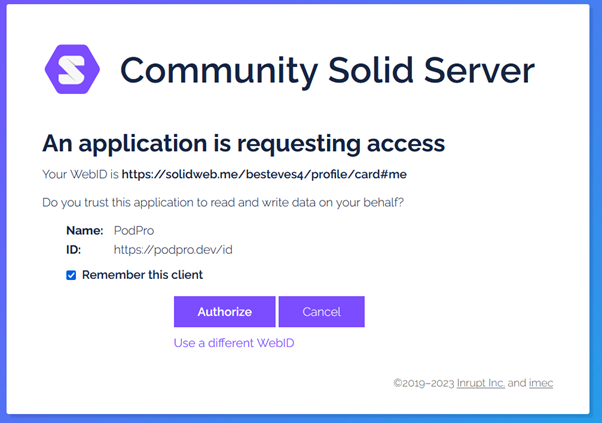
\includegraphics[width=0.4\linewidth]{figures/chapter-5/css.png}}
        \label{fig:css}
    }
    \qquad
    \subfigure[Enterprise Solid Server]{
        \fbox{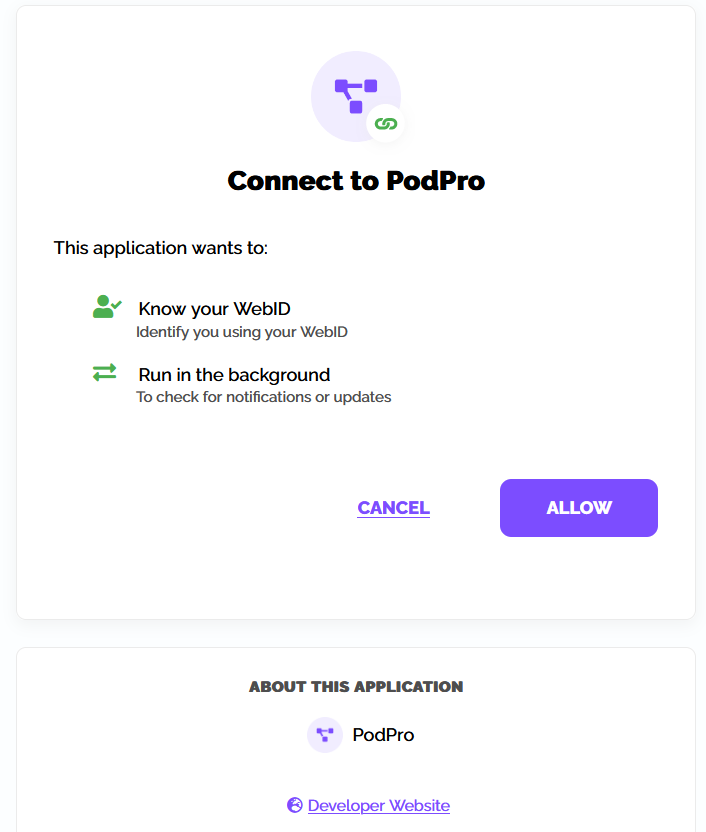
\includegraphics[width=0.4\linewidth]{figures/chapter-5/ess.png}}
        \label{fig:ess}
    }
\end{figure*}

\begin{figure}[htp]
    \centering
    \fbox{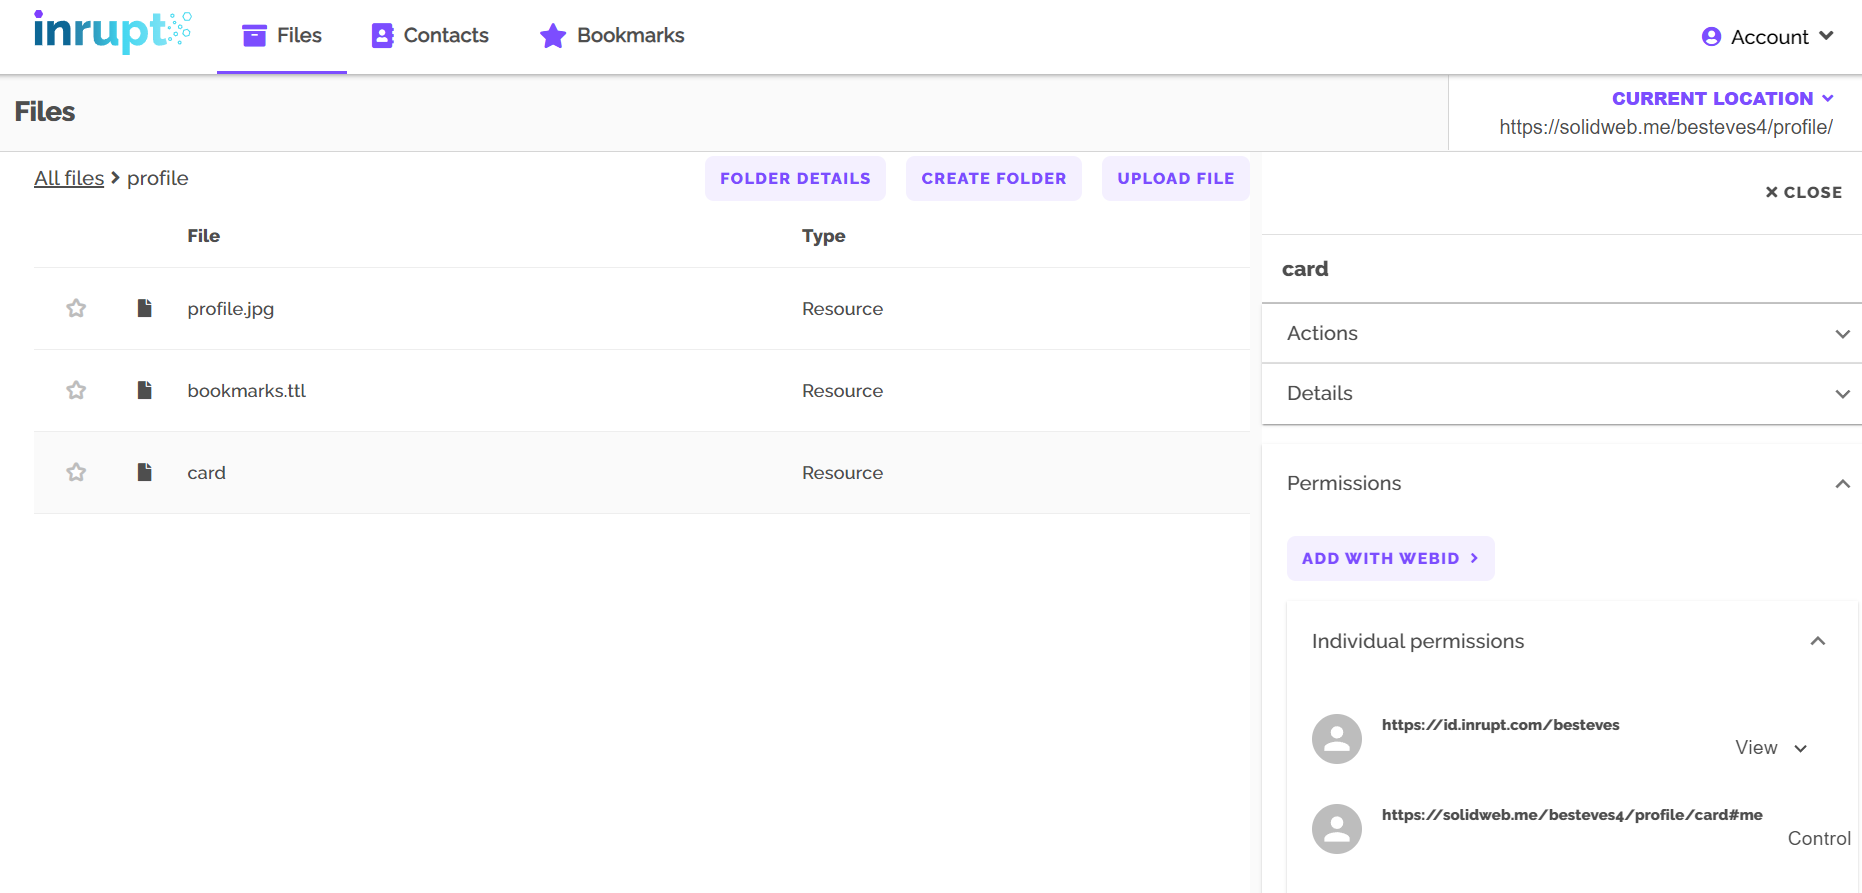
\includegraphics[width=0.9\linewidth]{figures/chapter-5/podbrowser.png}}
    \caption{Screenshot of Inrupt's PodBrowser app to manage data and access grants.}
    \label{fig:podbrowser}
\end{figure}

\begin{figure}[htp]
    \centering
    \fbox{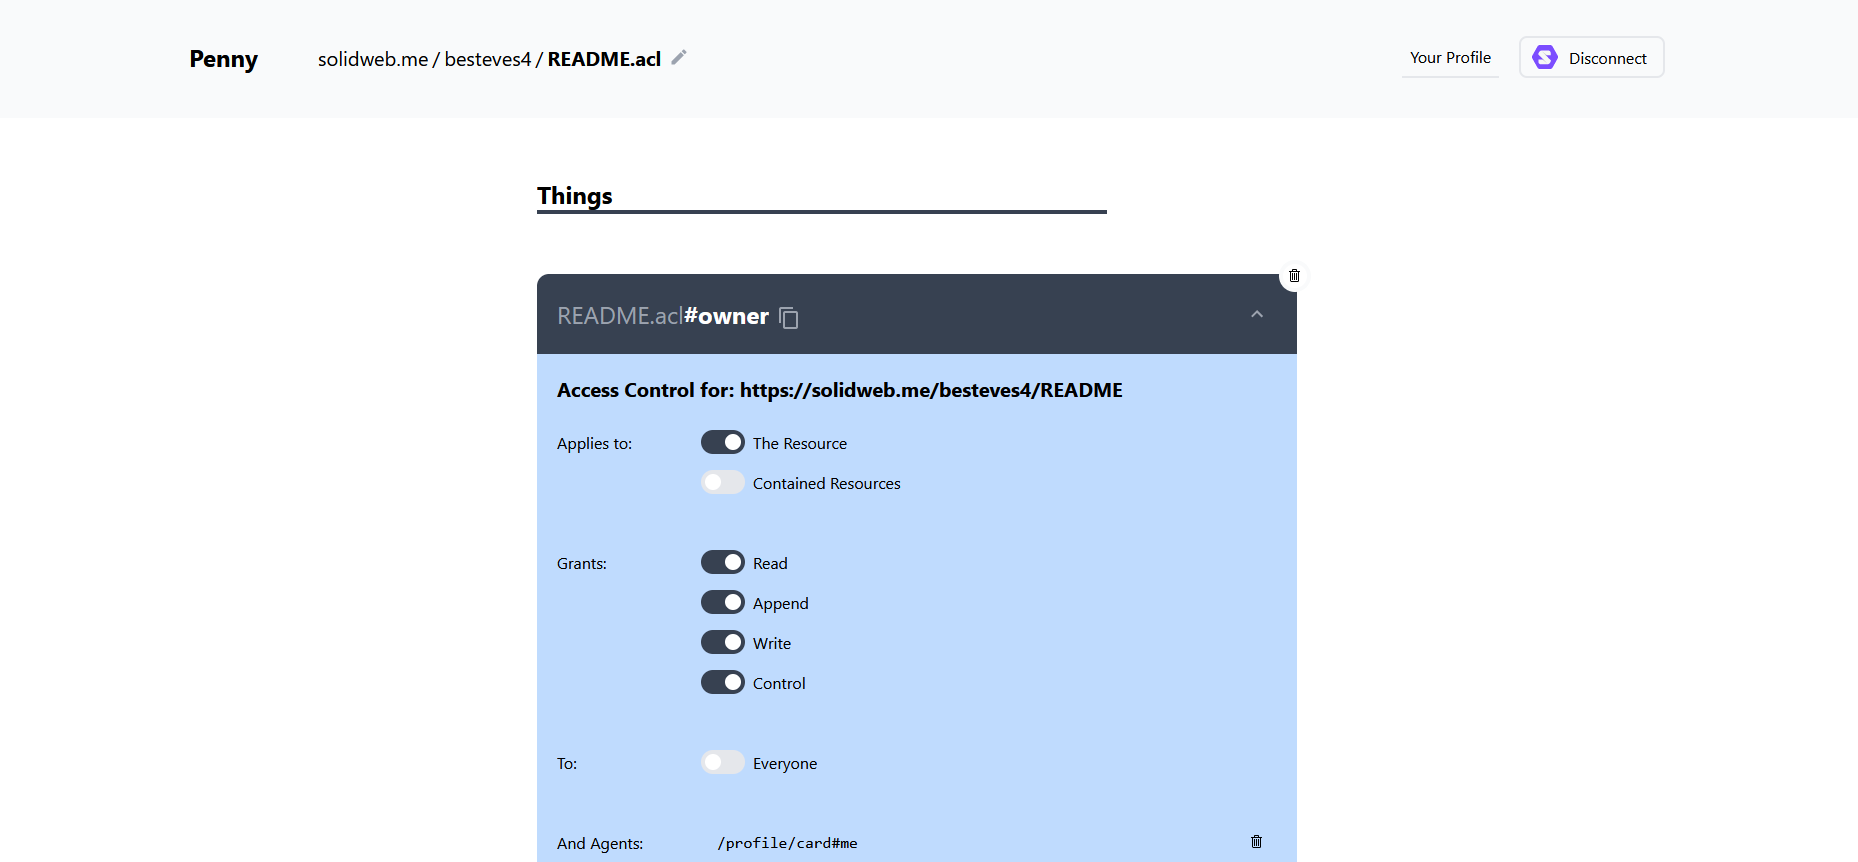
\includegraphics[width=0.9\linewidth]{figures/chapter-5/penny.png}}
    \caption{Screenshot of Penny app to manage data and access grants.}
    \label{fig:penny}
\end{figure}

Furthermore, two more legal challenges should be considered regarding the information obligations set out in the GDPR.
The first relates to how the information is presented to the data subject as GDPR Article 12 states that data controllers have an obligation to provide this information \textit{``in a concise, transparent, intelligible and easily accessible form, using clear and plain language''} \citeyearpar{noauthor_regulation_2016}.
As such, while the user's policies, others' requests and data access agreements can be easily accessed by data subjects if stored in Solid Pods, the implementation of interfaces to display the result of the policy matching process, especially the information that was previously unknown by the subject, might also be necessary to fully fulfil the requirements of Article 12 in ensuring that data subjects have read and understood this information.

The second challenge is related to the timing of the notification, as Articles 13 and 14 \citeyearpar{noauthor_regulation_2016} set different rules which depend on whether the data collection is done directly from the data subject or another entity.
As the GDPR does not directly mention data intermediary services, there is a gap that should be further explored to understand which Article applies in the Solid context.
On one hand, if the Pod provider is deemed a data controller, then the personal data is not directly collected from the data subject \citep{pandit_making_2023} and Article 14 applies, meaning that the data subject must be informed \textit{``at the latest at the time of the first communication to that data subject''} \citeyearpar{noauthor_regulation_2016}.
Access requests to Solid Pods can be considered to be communications with data subjects, and as such, at the time of the request, the information requirements should be fulfilled.
On the other hand, if the Pod provider is not thought to be a data controller, i.e., it is simply considered a piece of software used by the data subject, then the data is directly captured from the data subject and Article 13's \citeyearpar{noauthor_regulation_2016} requirements must be fulfilled at the time when said data is obtained.
Regardless, in both interpretations, the data subjects must be notified at the latest in the instant when the requests reach the data subjects' Pod.

%Both existing options to provide access in Solid can take distinct forms, as clearly stated by Figures~\ref{fig:authorisation-dialogue}, \ref{fig:podbrowser} and \ref{fig:penny}, also depending on the access control specification implemented in the server where the Pod is stored, since servers only have to comply with one access control protocol, i.e., WAC or ACP, as described in Section~\ref{sec:sota_solid}.

%FROM THE PAPER: The outcome of the matching exercise is a mapping between the user’s policies and the specifics of the request for accessing the data, emphasizing the differences between the two. This process can lower the burden of data subjects in reading and comprehending the information related to the processing of their personal data.

Additionally, the informed character of consent is only one of a series of requirements that must be met in order to obtain valid consent. 
After being informed, data subjects must state their preferences \textit{``by a statement or by a clear affirmative action''} \citeyearpar{noauthor_regulation_2016} which signifies their agreement with the handling of their personal data.
Moreover, EDPB's and WP 29's guidelines on consent \citep{european_data_protection_board_guidelines_2020,article_29_data_protection_working_party_opinion_2011,article_29_data_protection_working_party_article_2016} further develop the freely given, specific, informed and unambiguous characters of consent.
Among the discussed topics, these entities' guidelines state that consent must be granular, the data subjects must be aware of the consequences of refusing to consent and the distinct purposes for processing data must not be tied together.
Thus, simply accepting an access request does not necessarily signify consent according to the GDPR.

\subsection{Expressing consent in advance through OAC policies}
\label{sec:consent_advance}

The GDPR does not forbid the expression of consent in advance.
In fact, Recital 32 mentions that \textit{``Consent should be given by a clear affirmative act [...], such as by a written statement, including by electronic means, [...]. This could include ticking a box when visiting an internet website, choosing technical settings for information society services or another statement or conduct which clearly indicates in this context the data subject’s acceptance of the proposed processing of his or her personal data''} \citeyearpar{noauthor_regulation_2016}.
Nevertheless, in order for consent to be valid under the GDPR jurisdiction, it must be specific even for circumstances that may not have already happened \citep{kosta_consent_2013} and the data controllers must be able to demonstrate that \textit{``the data subject has, by active behaviour, given his or her consent to the processing of his or her personal data and that he or she has obtained, beforehand, information relating to all the circumstances surrounding that processing, in an intelligible and easily accessible form, using clear and plain language, allowing that person easily to understand the consequences of that consent, so that it is given with full knowledge of the facts''}, as stated in Case C-61/19 held in 2020 at the European Court of Justice \citeyearpar{noauthor_orange_2020}.
As such, in this Section, the usage of OAC policies to express the required GDPR terms to have valid consent are further explored. 
 
The automation of consent on the Web is not a new idea.
As a matter of fact, the Do Not Track (DNT)\footnote{\url{https://www.eff.org/issues/do-not-track} (accessed on 28 January 2024)} initiative and the previously described P3P are two examples in this respect.
Although none of these solutions have succeeded in being consumed at a large scale, they can be illustrative use cases of what to do -- and do not do -- while developing a system for Web consenting. 
The DNT initiative focused on blocking the ad-tech industry from tracking users based on their online behaviour by sending a signal from the users' browser to all Web pages they visited with the preference to not be tracked, similarly to the right to object asserted in GDPR Article 21, however it failed due to the lack of browser adoption and enforcement mechanisms \citep{kamara_not_2016}.
Similarly, the P3P initiative allowed Web pages to \textit{``express their privacy practices in a standard format that can be retrieved automatically and interpreted easily by user agents''} and \textit{``enable an expanded ecosystem in which web sites would consistently inform web user agents of personal data collection intentions and web users would configure their individual user agents to accept some practices automatically [...]''} \citep{cranor_platform_2002}.
However, one of P3P's main drawbacks was the lack of consistency between human and machine-readable privacy notices communicated to users \citep{cranor_web_2002}, a challenge which can also be attributed to Solid as the information presented to users in consent dialogues is not aligned with the authorisation statements stored in Solid Pods.
Moreover, WP 29 also stated that P3P had the capability of misleading data controllers into believing that they could be discharged of certain obligations as long as data subjects had already agreed to the processing of their data \citep{article_29_data_protection_working_party_article_2014}, an issue which can also very easily be relevant for the Solid ecosystem.

Nevertheless, Solid differs from P3P in the sense that it provides its users with a decentralised storage unit equipped with a permission-based access control mechanism, i.e., access to data is only provided in the presence of an authorisation for a particular application or user.
Furthermore, in such decentralised systems there is no need to transfer or make copies of data as access can be provided on demand to any user or application through its authorisation and authentication mechanisms, removing the need for such entities to keep copies of data in their own servers.
Said mechanisms can also serve as the starting point to keep access and usage logs in Solid Pods, which can be used by users and by external auditing entities to check whether Web services are using data according to their announced policies.
As such, users will have a more transparent overview of how their data is being used, which comes as an improvement over P3P’s lack of consistency and policy enforcement -- \textit{``no enforcement action followed when a site's policy expressed in P3P failed to reflect their actual privacy practices''} \citep{cranor_platform_2002} --, the main issues that led to its failure.
What's more, as previously stated in Section \ref{sec:sota_solid_data_protection}, there is ongoing research on the modelling of usage control policies \citep{akaichi_gucon_2023} and enforcement mechanisms for Solid \citep{slabbinck_rulebased_2023}.

% FROM PAPER: In a rather recent development, the Commissioner for Justice and Consumers, Didier Reynders, launched a reflection on how \replaced{better to}{to better} empower consumers to make effective choices regarding tracking-based advertising models \textls[-15]{({\url{https://commission.europa.eu/live-work-travel-eu/consumer-rights-and-complaints/enforcement-consumer-protection/cookie-pledge\_en}, accessed on 19/11/2023})}. The problem that it tries to solve is similar to the difficulties around accessing content in Solid Pods. 

The usage of pre-configured choices is also discussed in Recital 66 of Directive 2009/136/EC, the successor of the ePrivacy Directive \citeyearpar{noauthor_directive_2002}, which states that \textit{``Third parties may wish to store information on the equipment of a user, or gain access to information already stored, for a number of purposes, ranging from the legitimate (such as certain types of cookies) to those involving unwarranted intrusion into the private sphere (such as spyware or viruses). [...] Where it is technically possible and effective, [...] the user’s consent to processing may be expressed by using the appropriate settings of a browser or other application''} \citeyearpar{noauthor_directive_2009}.
This is also reflected on a few national implementations of the ePrivacy Directive that allow the indication of consent via technical means, e.g., Romania's Legea 506/2004 states that \textit{``the subscriber or user can use the settings of the internet browsing application or other similar technologies to delete stored information or to deny access to such information to third parties''} \citeyearpar{noauthor_legea_2004}.
However, the utility of browser settings to express consent is being challenged as recently the data protection authority in Finland ruled that \textit{``instructing website users to accept or decline to the use of cookies through browser settings does not constitute active and explicit consent under the GDPR''} \citep{fich_finland_2021}.
Nonetheless, several technical solutions to signal users' preferences have been emerging recently, e.g., the Global Privacy Control (GPC) \citep{global_privacy_control_gpc_2021} or the Advanced Data Protection Control (ADPC) \citep{human_advanced_2021} \textit{`privacy signals'}, which are still lacking adoption due to a lack of standardisation and legal approval towards the fulfilment of ePrivacy requirements \citep{santos_how_2023}.

In the next Section, the building blocks for consent automation are explored in detail, with a reflection on how OAC and Solid can be adapted to fulfil legal requirements. 